\documentclass[11pt]{ctexart}
\usepackage{amsmath,amssymb}
\usepackage[margin=1in]{geometry}
\usepackage{booktabs}
\usepackage{enumitem}
\usepackage{graphicx}
\usepackage{float}

\begin{document}

\title{线性回归分析 第6周作业实验报告}
\author{}
\date{}
\maketitle

% ======================================================================
\section*{Problem 1（KNNL 3.9）：电力消耗残差图}
% ======================================================================


\begin{figure}[H]
\centering
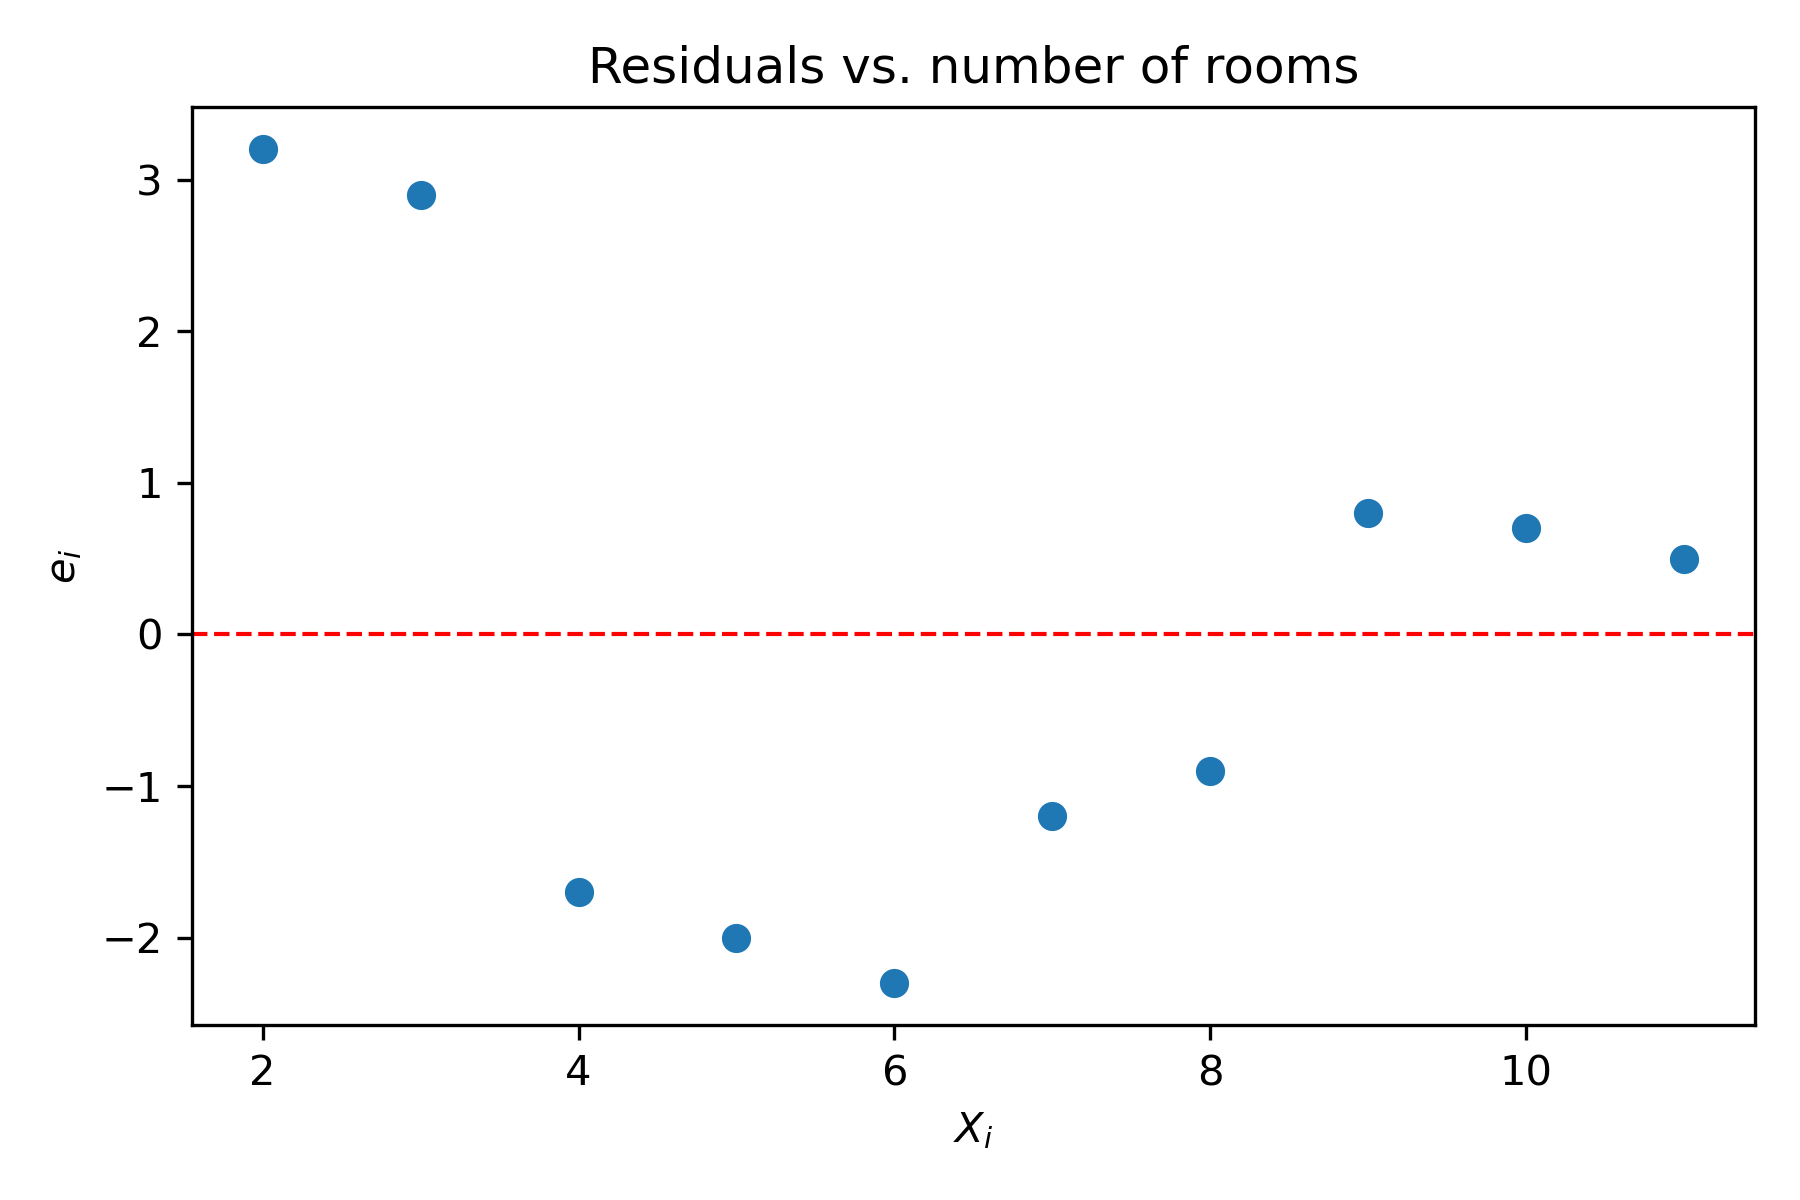
\includegraphics[width=0.72\linewidth]{figs/p1_resid_x.png}
\caption{残差 \(e_i\) 对房间数 \(X_i\) 的散点图}
\label{fig:p1}
\end{figure}

Nonlinearity and non-constant variance are evident in the residual plot. Some transformation such as quadratic might solve it.

% ======================================================================
\section*{Problem 2（KNNL 3.15）：溶液浓度}
% ======================================================================

\subsection*{(a) 线性回归拟合}

以时间为 \(X\)，浓度为 \(Y\)，拟合线性回归模型
\[
Y_i=\beta_0+\beta_1X_i+\varepsilon_i.
\]
由 \texttt{prob2.py} 输出，估计的线性回归函数为
\[
\hat Y=2.5753-0.3240X.
\]
即时间每增加 1 小时，溶液浓度平均下降约 \(0.3240\)。

\subsection*{(b) 失拟 \(F\) 检验}

检验假设为
\[
H_0:\ \text{线性回归函数是充分的，即不存在失拟},
\]
\[
H_1:\ \text{线性回归函数存在失拟}.
\]
取显著性水平 \(\alpha=0.025\)。

将总误差平方和分解为纯误差平方和与失拟平方和：
\[
SSE=SSPE+SSLF.
\]
由重复观测可得
\[
SSPE\approx 0.1574,\qquad df_{PE}=10,
\]
\[
SSE\approx 2.9246,\qquad df_E=15-2=13,
\]
因此
\[
SSLF=SSE-SSPE\approx 2.7672,\qquad df_{LF}=13-10=3.
\]
失拟检验统计量为
\[
F=\frac{SSLF/df_{LF}}{SSPE/df_{PE}}
=\frac{2.7672/3}{0.1574/10}
\approx 58.60.
\]
临界值为
\[
F_{0.975}(3,10)\approx 4.83.
\]
决策规则：若 \(F>F_{0.975}(3,10)\)，则拒绝 \(H_0\)。

由于
\[
F\approx 58.60>4.83,
\]
故在 \(\alpha=0.025\) 下拒绝 \(H_0\)，认为线性回归函数存在显著失拟，线性模型不合适。

\subsection*{(c)}

失拟检验只能说明“线性回归函数是否充分”。当检验拒绝 \(H_0\) 时，它只能告诉我们线性模型不合适，但不能直接指出应该采用哪一种回归函数。要确定合适的模型，还需要结合散点图、残差图、Box-Cox 变换、变量变换、多项式模型以及实际背景知识进行进一步分析。因此，即使失拟检验显著，也不能由该检验本身得到“应使用哪个模型”的结论。

% ======================================================================
\section*{Problem 3（KNNL 3.16）：变换与 Box-Cox 方法}
% ======================================================================

\subsection*{(a) 散点图与变换选择}

浓度 \(Y\) 对时间 \(X\) 的散点图见图 \ref{fig:p3scatter}。

\begin{figure}[H]
\centering
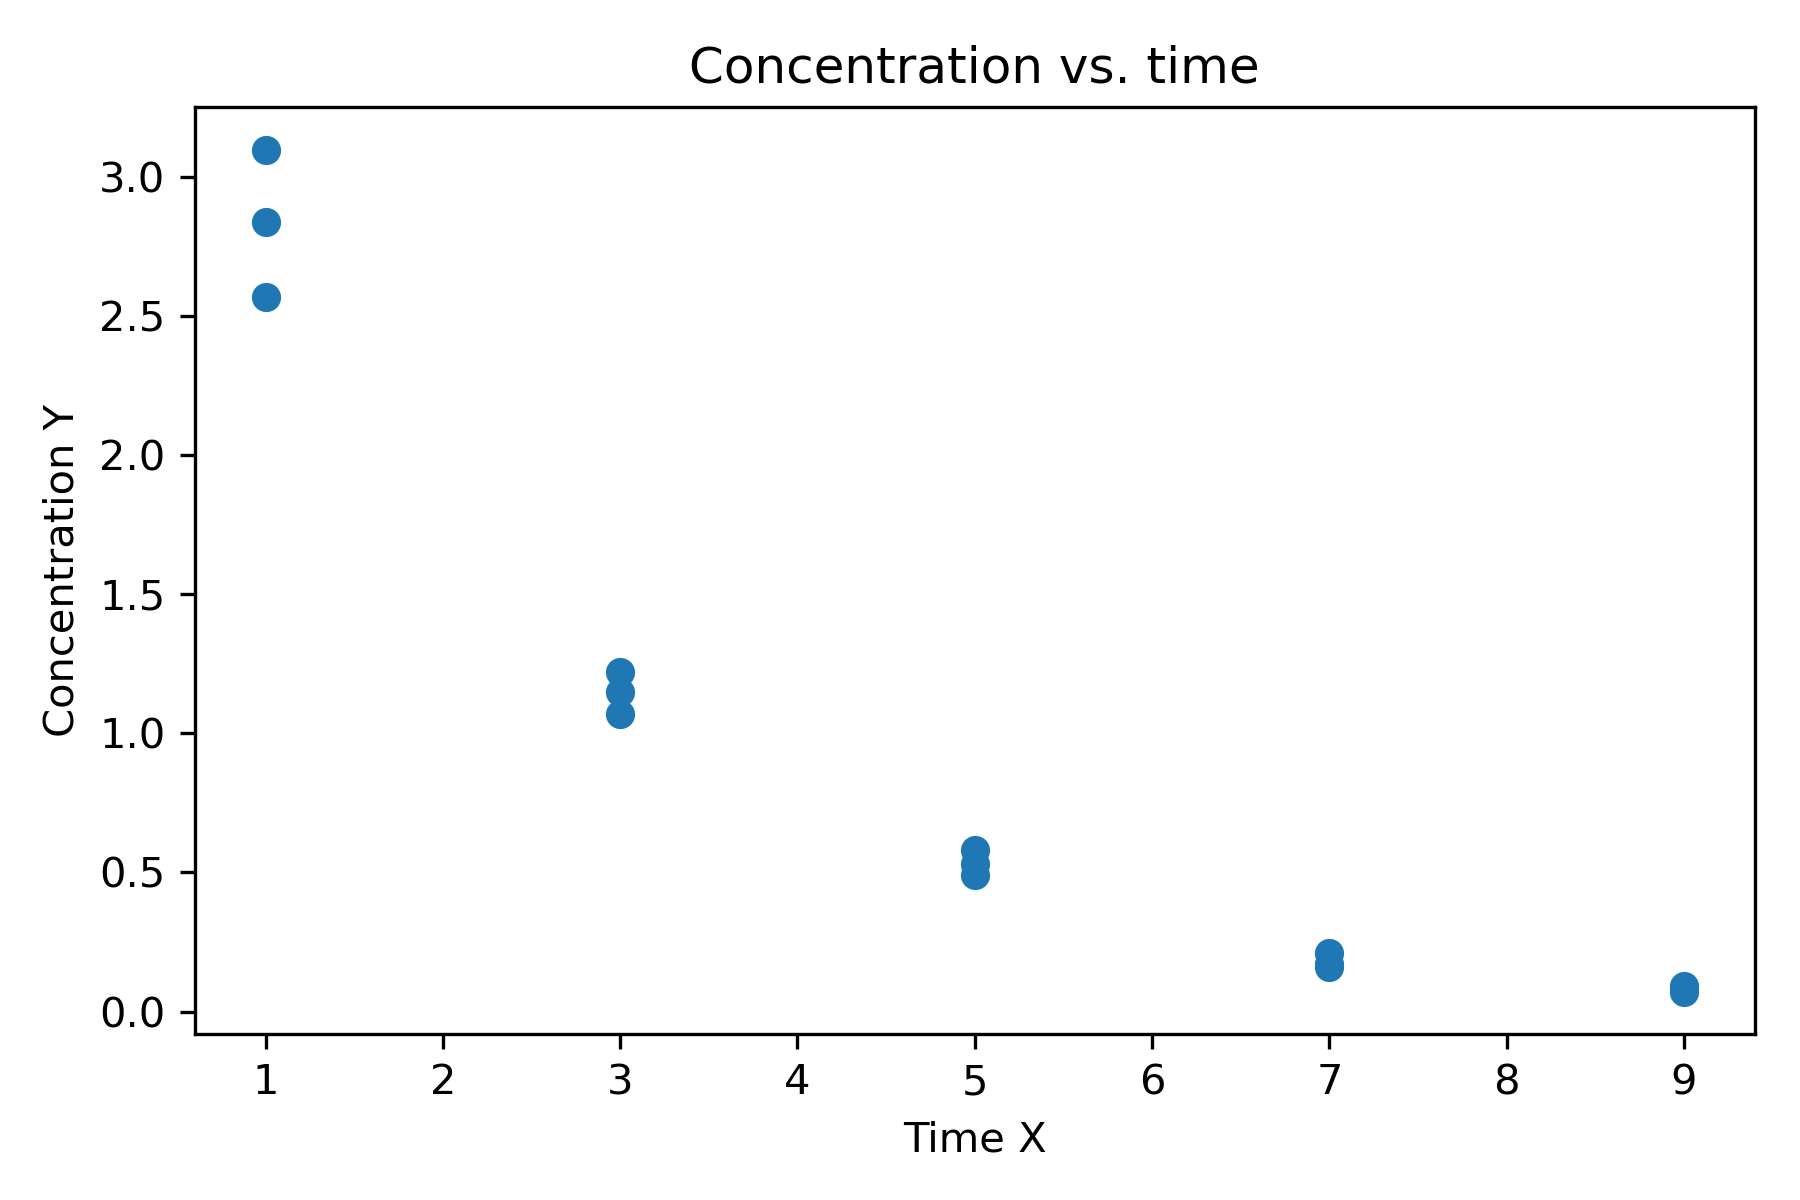
\includegraphics[width=0.72\linewidth]{figs/p3_scatter.png}
\caption{浓度 \(Y\) 对时间 \(X\) 的散点图}
\label{fig:p3scatter}
\end{figure}

图中 \(Y\) 随 \(X\) 增加而迅速下降，且下降速度逐渐变慢，同时不同时间点的离散程度随 \(Y\) 减小而减小。为了同时改善线性关系和方差稳定性，可以考虑对 \(Y\) 作对数变换。由化学浓度衰减的背景，也常用
\[
Y'=\log_{10}Y
\]
或自然对数变换。

\subsection*{(b) Box-Cox 标准化变换}

采用标准化 Box-Cox 变换
\[
Y_i'=
\begin{cases}
\dfrac{Y_i^\lambda-1}{\lambda g^{\lambda-1}}, & \lambda\neq 0,\\[1.2ex]
g\log Y_i, & \lambda=0,
\end{cases}
\]
其中 \(g=\exp\left(\frac{1}{n}\sum_{i=1}^n\log Y_i\right)\) 为几何平均值。

按题目要求，对
\[
\lambda=-0.2,\,-0.1,\,0,\,0.1,\,0.2
\]
分别进行变换并拟合线性模型 \(Y'=\beta_0+\beta_1X+\varepsilon\)，由 \texttt{prob3.py} 输出各 \(\lambda\) 对应的 \(SSE\)。运行结果整理为下表（精确值以程序输出为准）：

\begin{center}
\begin{tabular}{cc}
\toprule
\(\lambda\) & \(SSE\) \\
\midrule
\(-0.2\) & \(0.1207\) \\
\(-0.1\) & \(0.0646\) \\
\(0\)    & \(0.0390\) \\
\(0.1\)  & \(0.0441\) \\
\(0.2\)  & \(0.0788\) \\
\bottomrule
\end{tabular}
\end{center}

由表可见，\(SSE\) 在 \(\lambda=0\) 处达到最小，向两侧（\(\lambda=\pm0.1,\pm0.2\)）逐渐增大，因此 Box-Cox 准则建议取
\[
\lambda\approx 0,
\]
即对 \(Y\) 作对数变换。这与 Prob-3(a) 中散点图所提示的“对 \(Y\) 作对数变换以改善线性与方差稳定性”一致，也为 Prob-3(c) 中指定使用 \(Y'=\log_{10}Y\) 提供了依据。

\subsection*{(c) 使用 \(Y'=\log_{10}Y\) 拟合线性回归}

令
\[
Y'=\log_{10}Y.
\]
由 \texttt{prob3.py} 输出，估计的线性回归函数为
\[
\widehat{\log_{10}Y}=0.6549-0.1954X.
\]
因此变换后的拟合模型为
\[
\log_{10}\hat Y=0.6549-0.1954X.
\]

\subsection*{(d) 变换后数据与拟合直线}

变换后数据及拟合直线见图 \ref{fig:p3logfit}。

\begin{figure}[H]
\centering
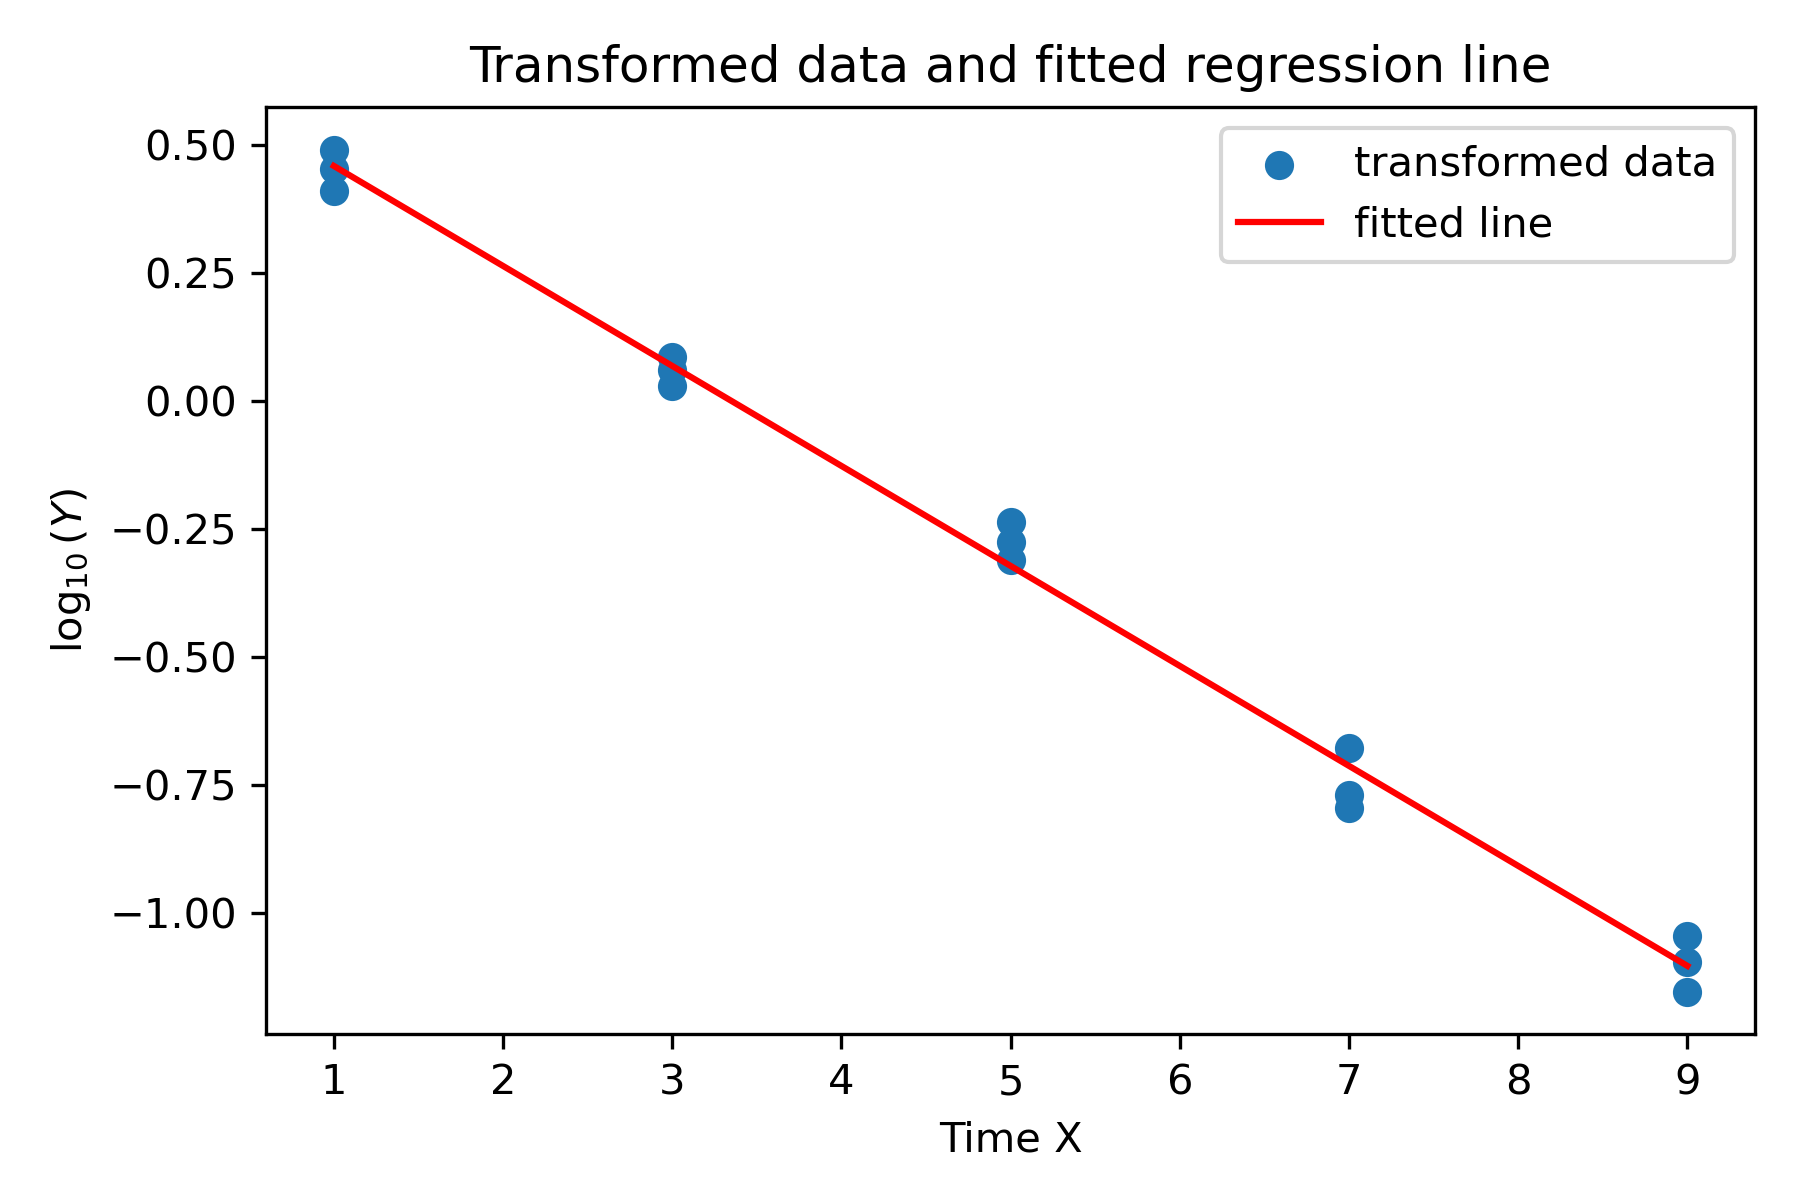
\includegraphics[width=0.72\linewidth]{figs/p3_logfit.png}
\caption{\(\log_{10}Y\) 对 \(X\) 的散点图及拟合直线}
\label{fig:p3logfit}
\end{figure}

从图可见，变换后的数据点大致围绕拟合直线分布，线性关系明显改善，拟合直线对变换后数据的拟合较好。

\subsection*{(e) 残差图与正态概率图}

残差对拟合值的图见图 \ref{fig:p3resid}，正态概率图见图 \ref{fig:p3qq}。

\begin{figure}[H]
\centering
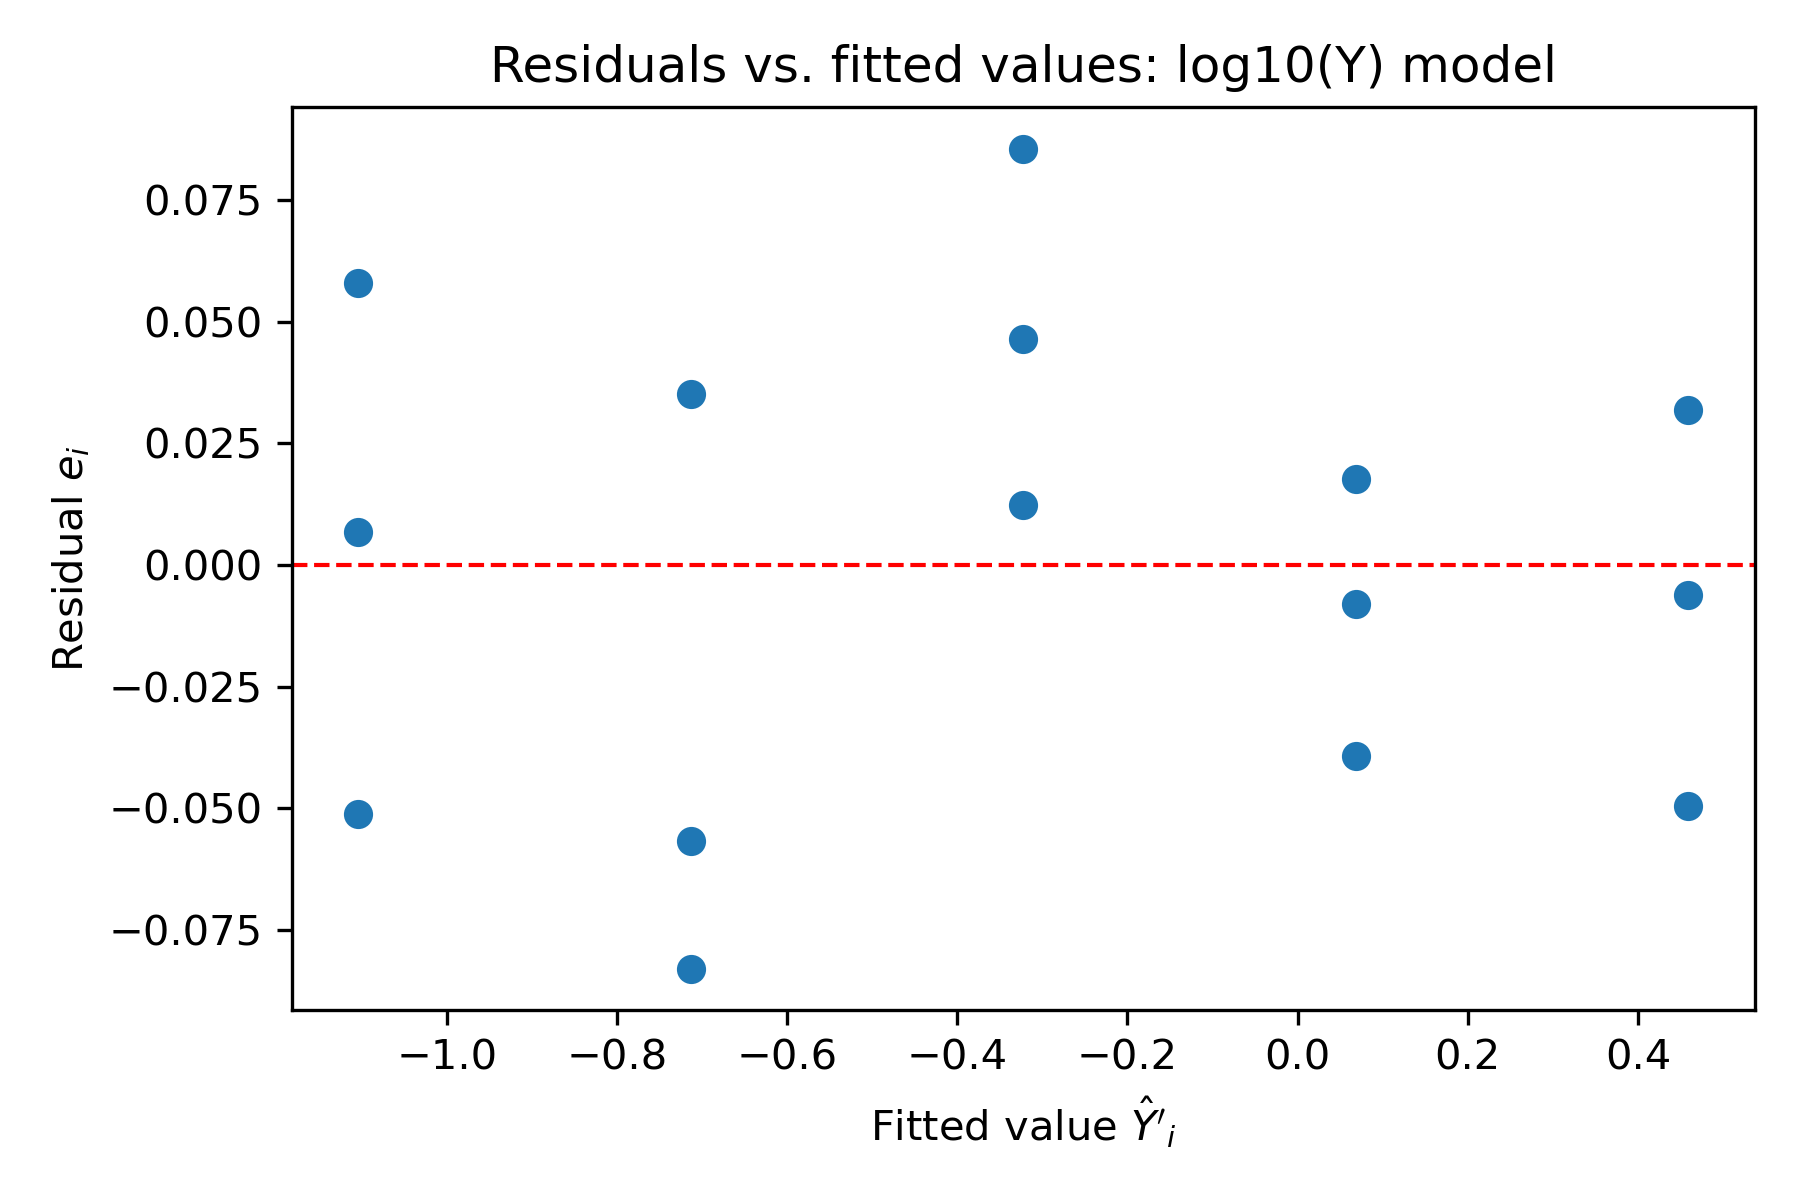
\includegraphics[width=0.72\linewidth]{figs/p3_resid_fit.png}
\caption{\(\log_{10}Y\) 模型的残差对拟合值图}
\label{fig:p3resid}
\end{figure}

\begin{figure}[H]
\centering
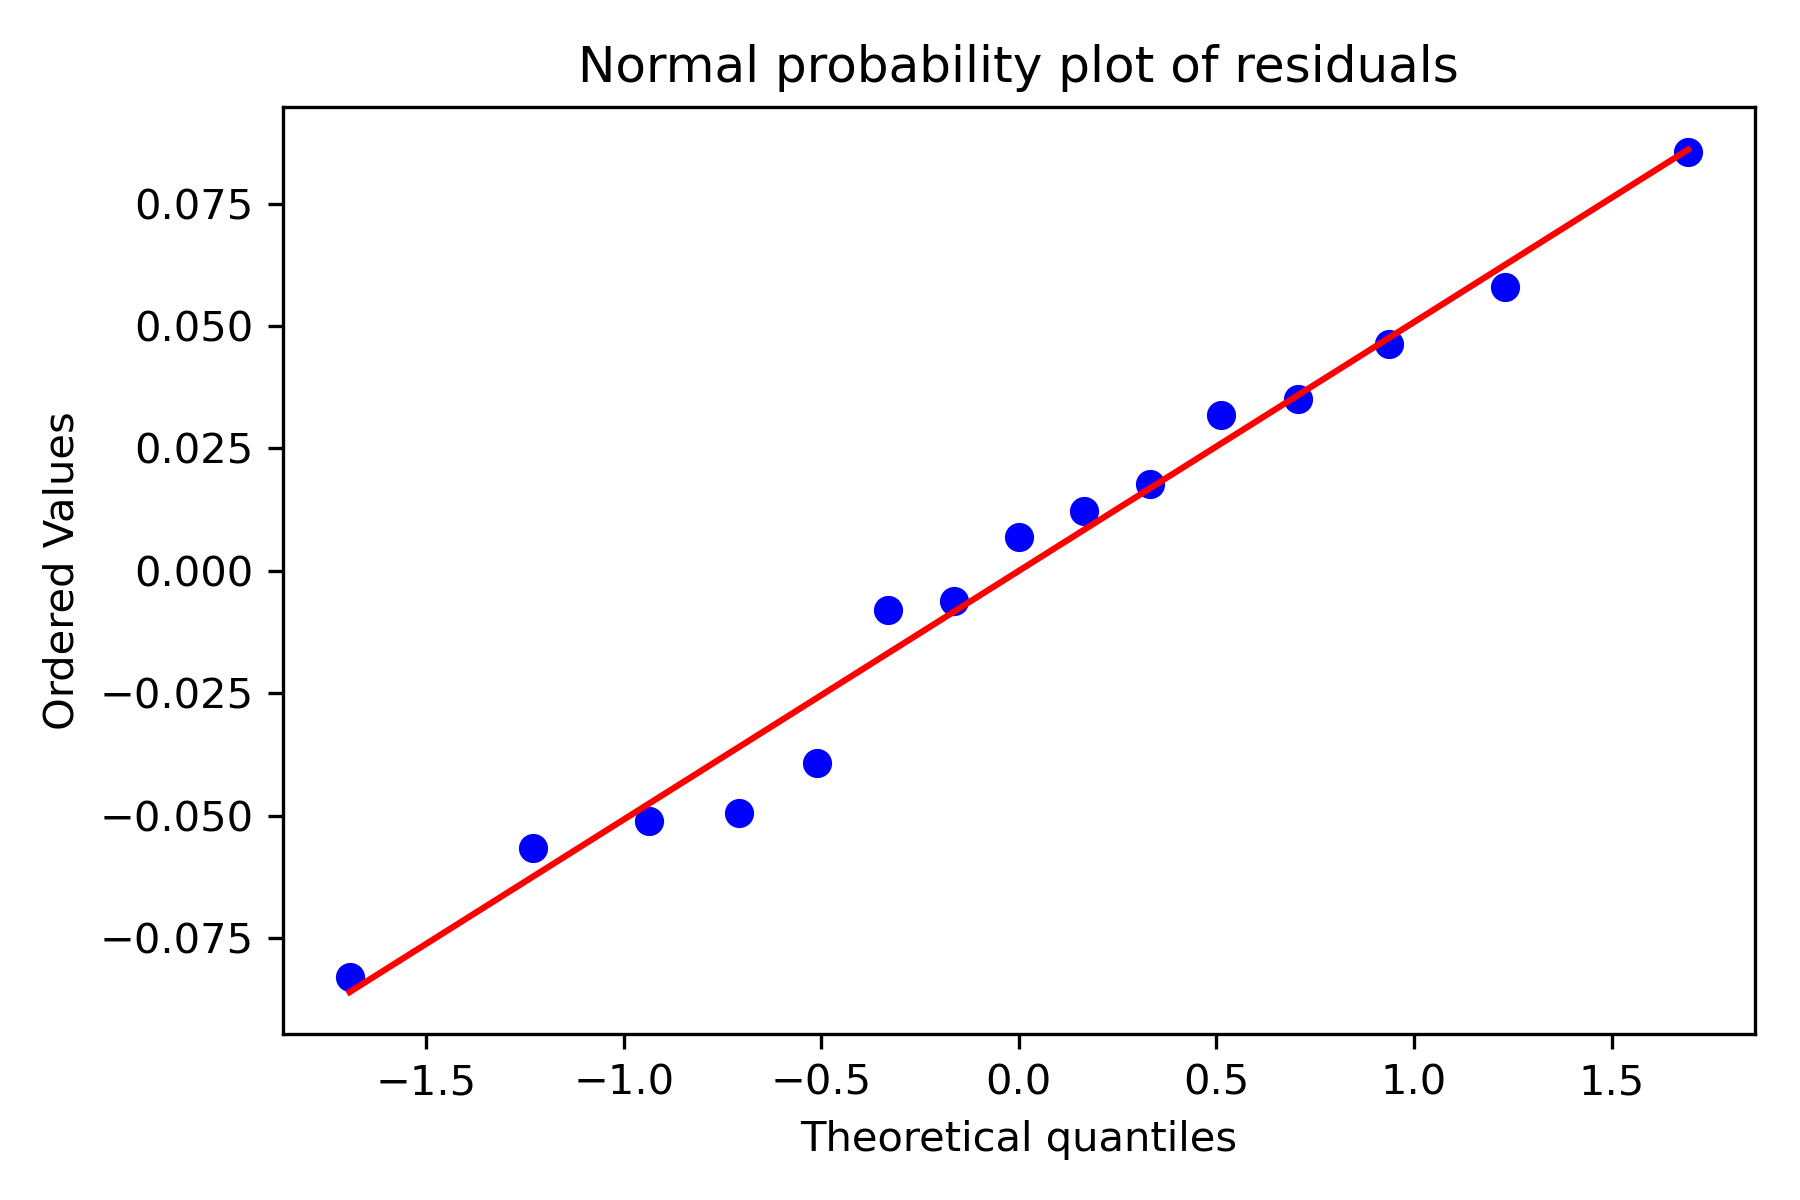
\includegraphics[width=0.72\linewidth]{figs/p3_qq.png}
\caption{\(\log_{10}Y\) 模型残差的正态概率图}
\label{fig:p3qq}
\end{figure}

残差图未显示明显的系统弯曲趋势，说明对数变换后线性关系基本合理。正态概率图整体接近直线，说明残差正态性假定没有明显违背。个别点可能略有偏离，但总体未见严重异常。

\subsection*{(f) 还原到原始单位}

由于
\[
\log_{10}\hat Y=0.6549-0.1954X,
\]
还原到原始单位得
\[
\hat Y=10^{\,0.6549-0.1954X}.
\]
这就是原始单位下的估计回归函数。

% ======================================================================
\section*{Problem 4：Michaelis--Menten 模型的线性化}
% ======================================================================

Michaelis--Menten 模型为
\[
V=\frac{\theta_1 C}{\theta_2+C}.
\]
取倒数得
\[
\frac{1}{V}=\frac{1}{\theta_1}+\frac{\theta_2}{\theta_1}\frac{1}{C}
=\beta_0+\beta_1\frac{1}{C}.
\]

\subsection*{(a) \(V\) 对 \(C\) 的散点图}

\(V\) 对 \(C\) 的散点图见图 \ref{fig:p4vc}。

\begin{figure}[H]
\centering
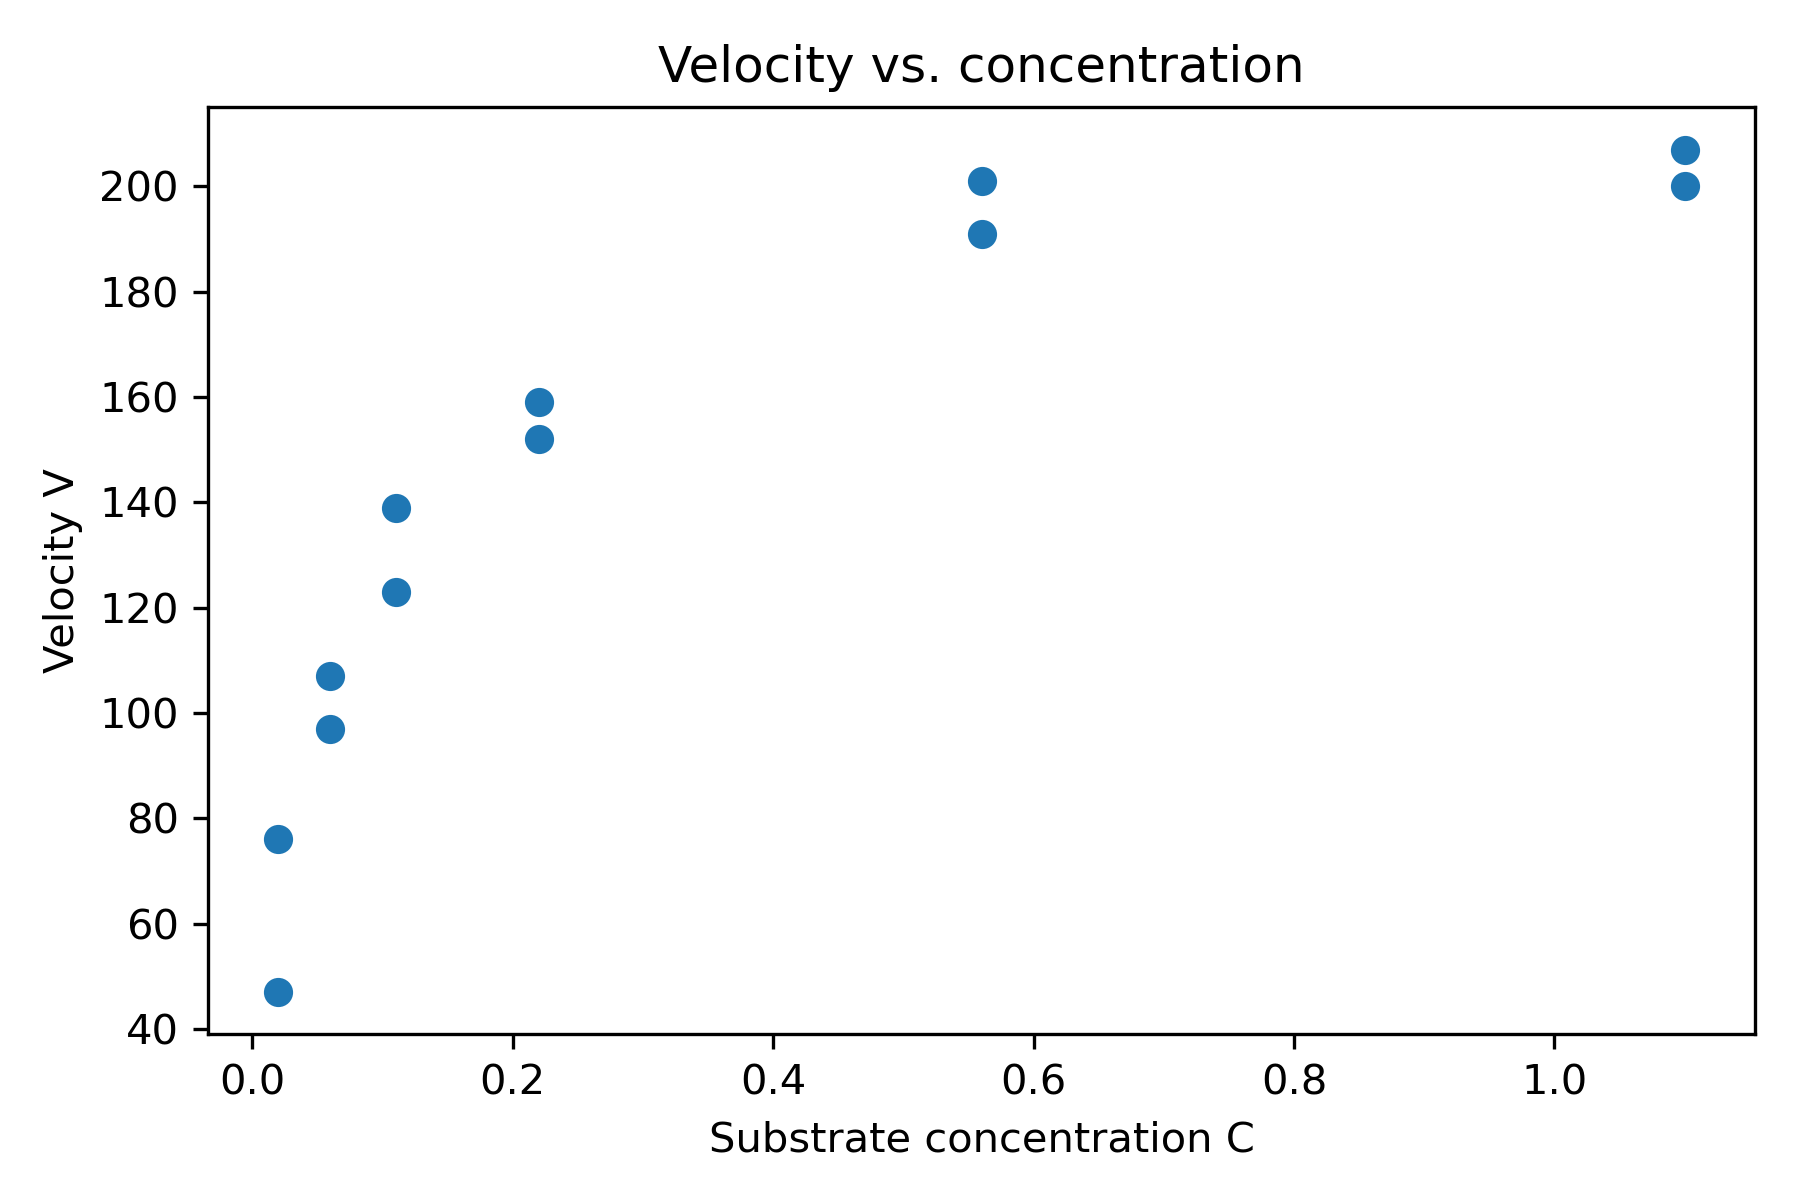
\includegraphics[width=0.72\linewidth]{figs/p4_vc.png}
\caption{速度 \(V\) 对浓度 \(C\) 的散点图}
\label{fig:p4vc}
\end{figure}

图形呈现明显的非线性饱和形态：随着 \(C\) 增大，\(V\) 先快速增加，随后逐渐趋于平台。这与 Michaelis--Menten 模型的理论形状一致。

\subsection*{(b) \(1/V\) 对 \(1/C\) 的散点图}

令
\[
C'=\frac{1}{C},\qquad V'=\frac{1}{V}.
\]
\(1/V\) 对 \(1/C\) 的散点图见图 \ref{fig:p4inv}。

\begin{figure}[H]
\centering
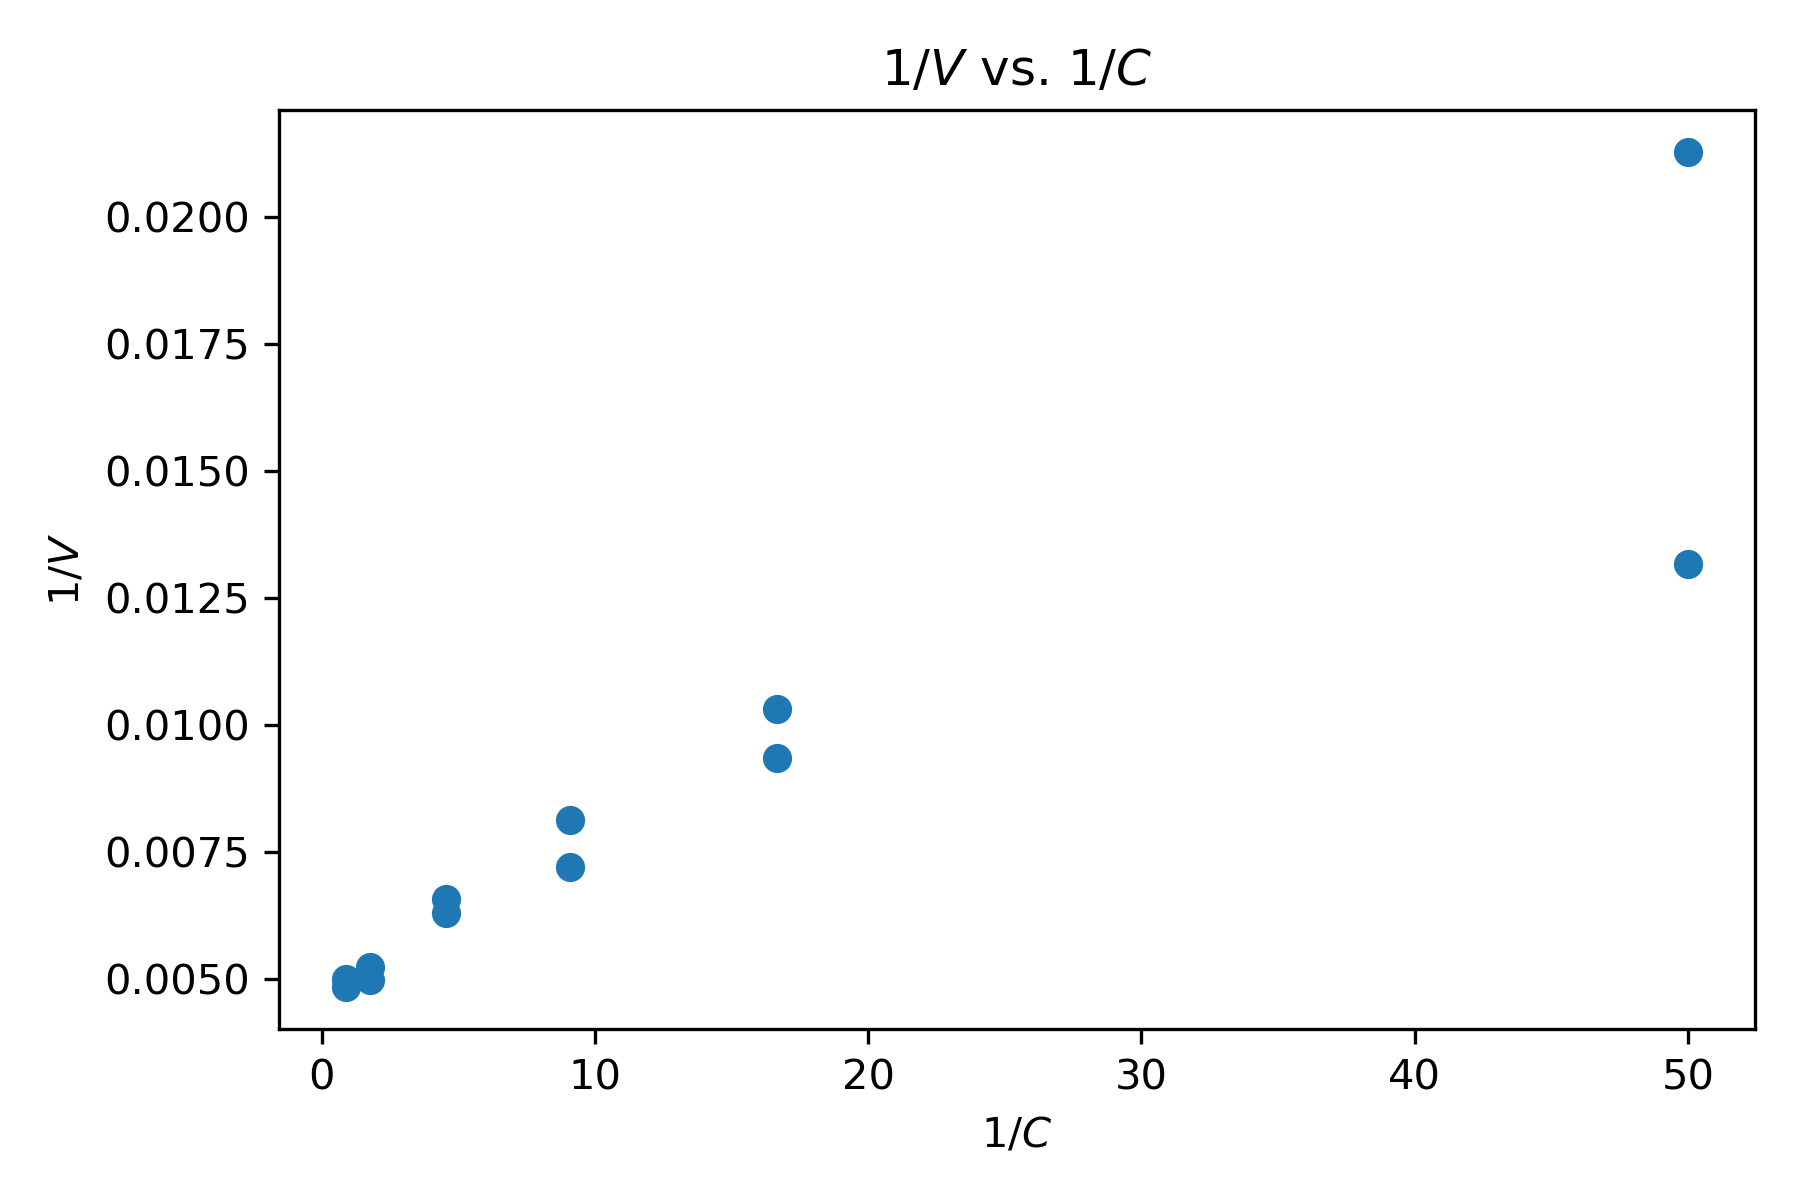
\includegraphics[width=0.72\linewidth]{figs/p4_inv.png}
\caption{\(1/V\) 对 \(1/C\) 的散点图}
\label{fig:p4inv}
\end{figure}

从图可见，变换后的点大致呈线性关系，说明线性化模型在均值结构上基本合理。但由于 \(1/C\) 在 \(C\) 较小时会被放大，因此小浓度点可能具有较高杠杆，且残差方差可能不完全相等。

\subsection*{(c) \(1/C\) 的分布与影响点}

\(1/C\) 与 \(C\) 的分布明显不同：取倒数会强烈拉伸较小的 \(C\) 值。因此 \(C\) 很小的观测在 \(1/C\) 尺度上会变成很大的解释变量值，可能具有较高杠杆和较大影响。由 \texttt{prob4.py} 输出的杠杆值 \(h_{ii}\) 和 Cook 距离可识别影响点；通常最小浓度附近的点更可能成为强影响点。

\subsection*{(d) \(1/V\) 对 \(1/C\) 的最小二乘回归与残差图}

由 \texttt{prob4.py} 输出，估计的线性化回归函数为
\[
\widehat{\frac{1}{V}}
\approx 0.005108+0.0002472\frac{1}{C}.
\]
残差对拟合值的图见图 \ref{fig:p4resid}。

\begin{figure}[H]
\centering
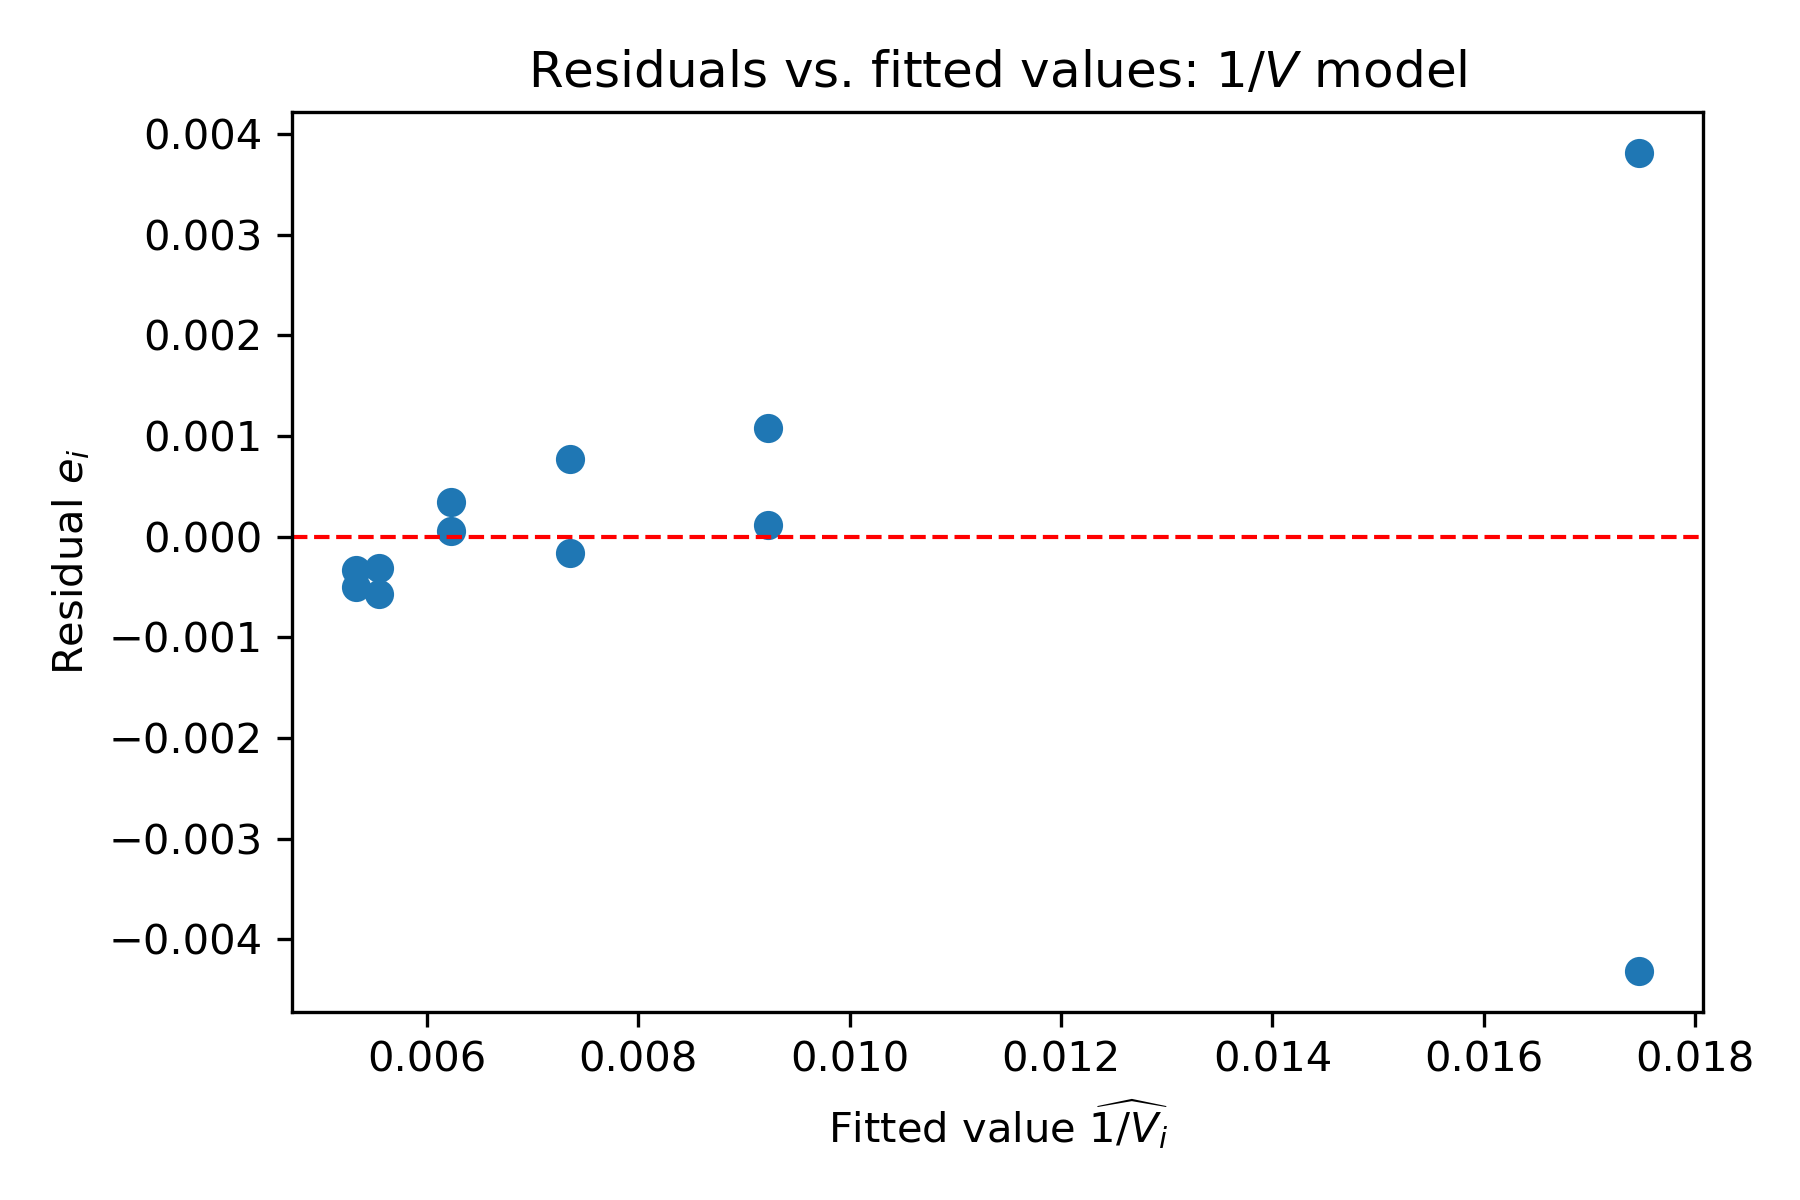
\includegraphics[width=0.72\linewidth]{figs/p4_resid.png}
\caption{\(1/V\) 模型的残差对拟合值图}
\label{fig:p4resid}
\end{figure}

不同方差，有漏斗形。

\subsection*{(e) 还原为原始单位并比较拟合}

由
\[
\frac{1}{V}=\beta_0+\beta_1\frac{1}{C},
\]
可得原始单位下的预测为
\[
\hat V=\frac{1}{\hat\beta_0+\hat\beta_1/C}.
\]
将观测点 \(V\) 对 \(C\) 与预测曲线同时画出，见图 \ref{fig:p4fit}。

\begin{figure}[H]
\centering
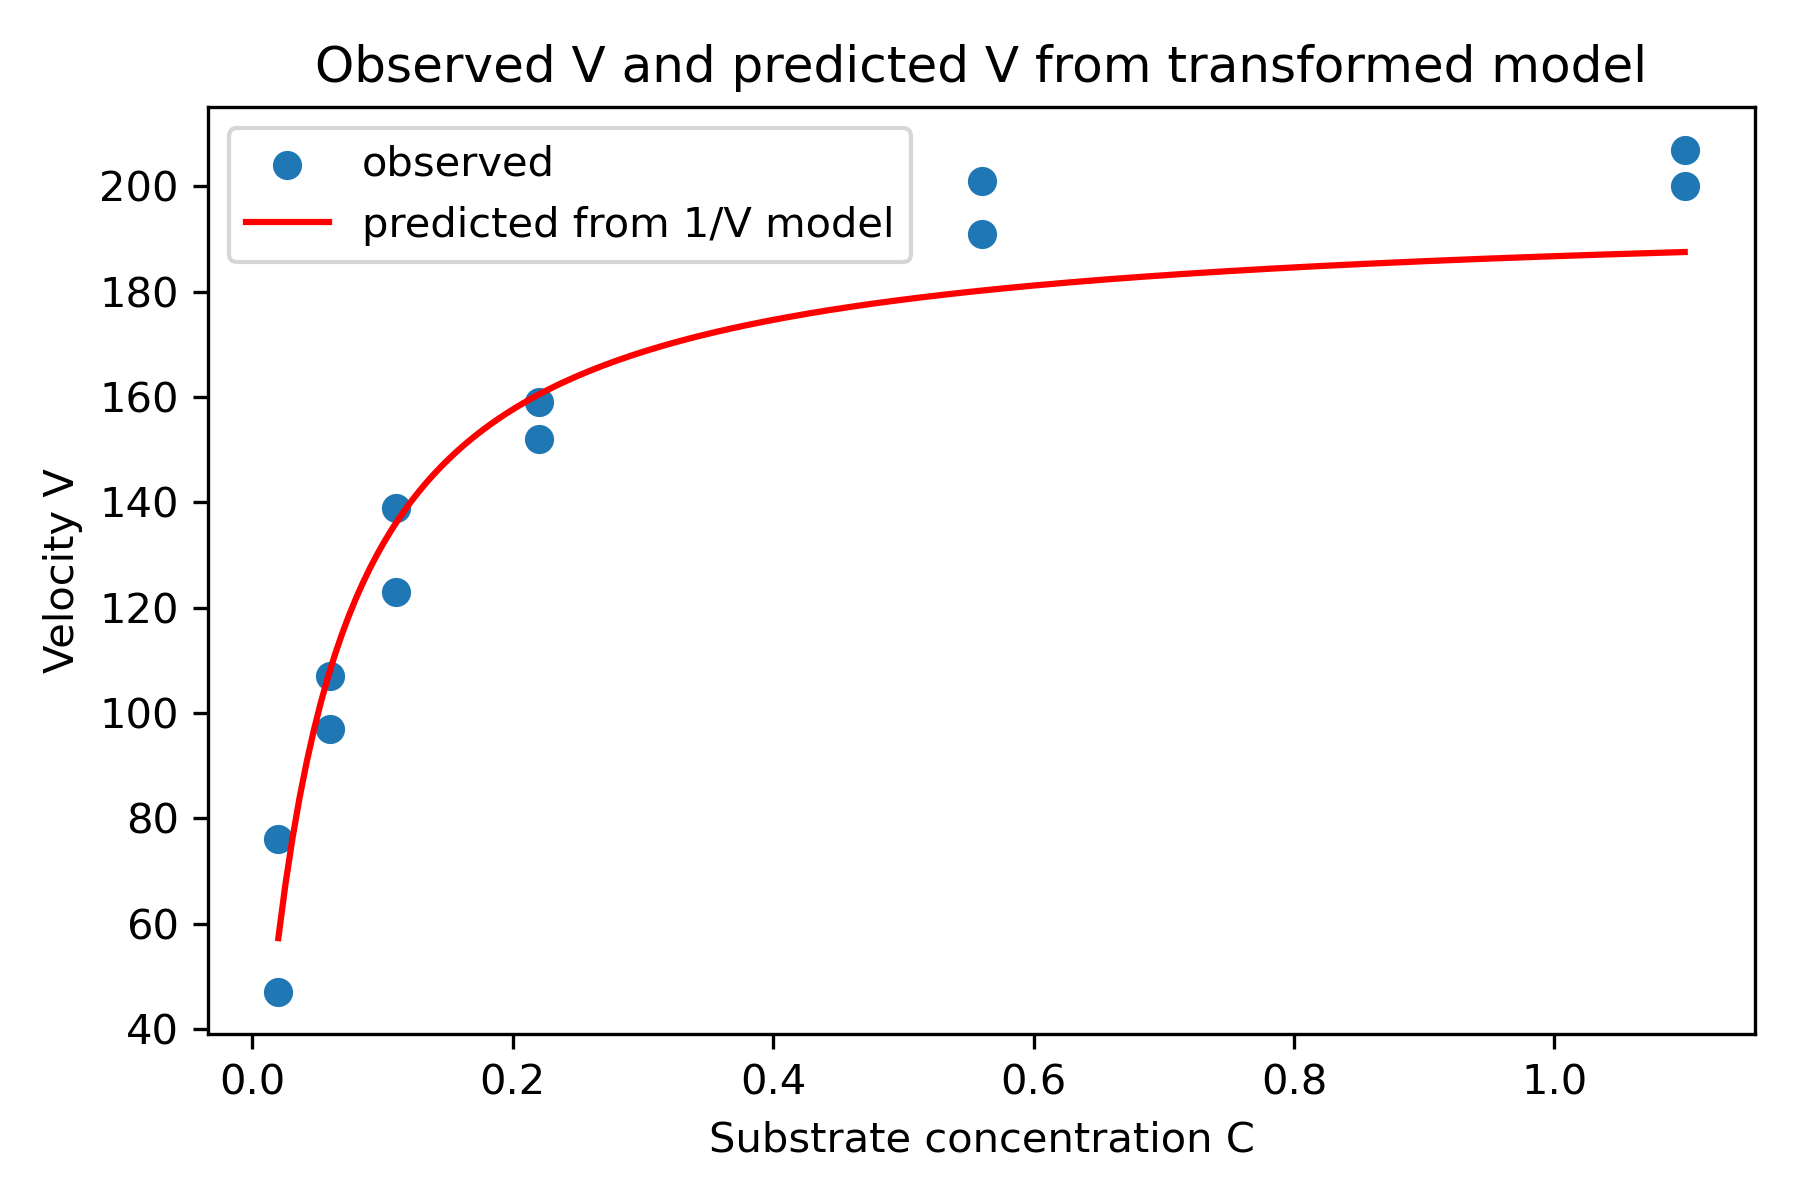
\includegraphics[width=0.72\linewidth]{figs/p4_vc_fit.png}
\caption{原始尺度下观测 \(V\) 与由线性化模型还原的预测曲线}
\label{fig:p4fit}
\end{figure}

从图可见，线性化模型还原后的曲线能够刻画 \(V\) 随 \(C\) 增加并趋于饱和的整体趋势。但若小 \(C\) 点影响较大，则原始尺度下的拟合可能在低浓度区域存在一定偏差。因此，线性化方法可以作为初步分析，但若需要更严格的推断，可进一步考虑非线性最小二乘拟合 Michaelis--Menten 模型。

\end{document}